% Part III-B, results (included by main_en.tex).
% DRAFT, written with seed 1 of the four conditions; every claim is to be checked against both seeds.

\section{Results}\label{sec:res}

Each condition ran with \NUM{seeds_subkev} seeds of 200 steps; Part II's \texttt{rlvr}, which labels every completion,
is the reference with the full label budget (\NUM{seeds_rlvr} seeds). Table~\ref{tab:sub-acc} gives the final policies'
accuracies and Table~\ref{tab:sub-paired} the paired differences to \texttt{rlvr\_sub}, the condition that simply drops
the unlabelled completions. Table~\ref{tab:sub-fill} shows how good each fill-in reward was on the completions it
scored, Table~\ref{tab:sub-style} what the final policies write, and Figure~\ref{fig:sub-curves} the training curves.
The intervals resample problems and do not include the variation between seeds.

\begin{table}[t]
\centering\small
\begin{tabular}{@{}lcccccc@{}}
\toprule
condition & seeds & MATH-500 & GSM8K & AMC23 & AIME24 & AIME25 \\ \midrule
base model & -- & 76.5 & 87.9 & 50.6 & 10.0 & 10.9 \\ \midrule
\texttt{rlvr} & 3 & 82.5 $\pm$ 0.6 & 93.0 $\pm$ 0.3 & 60.9 $\pm$ 2.4 & 21.5 $\pm$ 0.4 & 16.7 $\pm$ 2.1 \\
\texttt{rlvr\_sub} & 2 & 81.8 $\pm$ 1.7 & 92.4 $\pm$ 0.4 & 60.8 $\pm$ 1.1 & 18.3 $\pm$ 1.8 & 15.4 $\pm$ 0.3 \\
\texttt{sub\_kev} & 2 & 79.5 $\pm$ 1.3 & 91.2 $\pm$ 1.3 & 56.1 $\pm$ 3.5 & 15.9 $\pm$ 1.6 & 14.5 $\pm$ 1.6 \\
\texttt{sub\_kev\_recal} & 2 & 81.2 $\pm$ 2.5 & 92.3 $\pm$ 0.9 & 59.4 $\pm$ 1.8 & 21.1 $\pm$ 4.6 & 14.7 $\pm$ 3.4 \\
\texttt{sub\_probe} & 2 & 85.9 $\pm$ 1.8 & 93.7 $\pm$ 0.5 & 67.7 $\pm$ 2.3 & 30.5 $\pm$ 0.1 & 23.9 $\pm$ 1.3 \\
\bottomrule
\end{tabular}

\caption{Final policies: accuracy in percent, seed mean $\pm$ standard deviation over seeds. MATH-500 and GSM8K: greedy.
AMC23, AIME24 and AIME25: mean over 16 samples per problem at temperature 0.6. \texttt{rlvr}: every completion labelled
(Part II); the other conditions label 2 of the 8 completions of each group.}
\label{tab:sub-acc}
\end{table}

\paragraph{Dropping three quarters of the labels costs a little.} With only the two labelled completions of each group,
\texttt{rlvr\_sub} reaches \NUM{acc_sub_math}\% on MATH-500. Labelling all eight (\texttt{rlvr}) gives
\NUM{d_rlvr_math} \ci{\NUM{dlo_rlvr_math}}{\NUM{dhi_rlvr_math}} points more, and \NUM{d_rlvr_aime24}
\ci{\NUM{dlo_rlvr_aime24}}{\NUM{dhi_rlvr_aime24}} on AIME24. A fill-in reward has this much to win back.

\begin{table}[t]
\centering\small
\begin{tabular}{@{}lccccc@{}}
\toprule
minus \texttt{rlvr\_sub} & MATH-500 & GSM8K & AMC23 & AIME24 & AIME25 \\ \midrule
\texttt{rlvr} & $+$0.7 & $+$0.6 & $+$0.1 & $+$3.2 & $+$1.3 \\
 & {\footnotesize \ci{$-$1.1}{2.7}} & {\footnotesize \ci{$-$0.2}{1.4}} & {\footnotesize \ci{$-$3.2}{3.3}} & {\footnotesize \ci{1.0}{5.7}} & {\footnotesize \ci{$-$0.7}{3.3}} \\[2pt]
\texttt{sub\_kev} & $-$2.3 & $-$1.2 & $-$4.7 & $-$2.4 & $-$0.9 \\
 & {\footnotesize \ci{$-$4.4}{$-$0.1}} & {\footnotesize \ci{$-$2.1}{$-$0.2}} & {\footnotesize \ci{$-$8.8}{$-$0.3}} & {\footnotesize \ci{$-$5.3}{0.1}} & {\footnotesize \ci{$-$4.2}{2.2}} \\[2pt]
\texttt{sub\_kev\_recal} & $-$0.6 & $+$0.0 & $-$1.4 & $+$2.8 & $-$0.7 \\
 & {\footnotesize \ci{$-$2.8}{1.6}} & {\footnotesize \ci{$-$0.9}{0.8}} & {\footnotesize \ci{$-$5.5}{3.2}} & {\footnotesize \ci{0.8}{5.2}} & {\footnotesize \ci{$-$3.1}{1.4}} \\[2pt]
\texttt{sub\_probe} & $+$4.1 & $+$1.3 & $+$7.0 & $+$12.2 & $+$8.4 \\
 & {\footnotesize \ci{1.6}{6.6}} & {\footnotesize \ci{0.4}{2.3}} & {\footnotesize \ci{2.7}{11.2}} & {\footnotesize \ci{5.2}{20.3}} & {\footnotesize \ci{4.0}{13.5}} \\[2pt]
\bottomrule
\end{tabular}

\caption{Paired differences to \texttt{rlvr\_sub}, in percentage points: per problem, each condition's seed mean,
averaged over problems, with a 95\% bootstrap interval over problems.}
\label{tab:sub-paired}
\end{table}

\paragraph{The frozen judge makes things worse.} Rewarding the unlabelled completions with \kev{}'s $\pc$ as released
(\texttt{sub\_kev}) ends below dropping them: \NUM{d_subkev_math} \ci{\NUM{dlo_subkev_math}}{\NUM{dhi_subkev_math}}
points on MATH-500, \NUM{d_subkev_gsm} \ci{\NUM{dlo_subkev_gsm}}{\NUM{dhi_subkev_gsm}} on GSM8K, \NUM{d_subkev_amc}
\ci{\NUM{dlo_subkev_amc}}{\NUM{dhi_subkev_amc}} on AMC23 and \NUM{d_subkev_aime24}
\ci{\NUM{dlo_subkev_aime24}}{\NUM{dhi_subkev_aime24}} on AIME24. Yet the judge kept ranking the unlabelled completions
well: its AUROC for the withheld labels was \NUM{fillauc_all_subkev} over the run (Table~\ref{tab:sub-fill}). It was
too generous from the start, though. Its mean $\pc$ on the unlabelled completions was \NUM{fillmean_first20_subkev} in
the first 20 steps, when \NUM{unlacc_first20_subkev}\% of them were correct, and \NUM{fillmean_last20_subkev} in the
last 20, when \NUM{unlacc_last20_subkev}\% were. Which completions are labelled is random, so a constant offset raises
the expected reward of every behaviour by the same amount, which the group baseline removes in expectation. A judge
that pays more for some behaviour than its correctness warrants changes what the policy learns. By the end the policy repeats itself:
\NUM{srep_subkev} of the lines of its MATH-500 solutions repeat an
earlier line, against
\NUM{srep_sub} for \texttt{rlvr\_sub}, and \NUM{strunc_subkev} of the solutions run into the 2048-token limit
(Table~\ref{tab:sub-style}). After its first answer it restates its conclusion again and again, often until the
length limit. That does not change the answer the verifier reads, so the labelled completions do not punish it, and on
the unlabelled ones the judge pays for it (\S\ref{sec:res-repeat}).

\begin{table}[t]
\centering\small
\begin{tabular}{@{}lcccccccc@{}}
\toprule
 & & \multicolumn{3}{c}{fill-in AUROC} & frozen \kev{} & & \multicolumn{2}{c}{mean} \\ \cmidrule(lr){3-5}\cmidrule(l){8-9}
condition & seeds & steps 0--19 & first half & second half & AUROC & ECE & fill-in & label \\ \midrule
\texttt{sub\_kev} & 2 & 0.89 & 0.92 & 0.90 & 0.91 & 0.19 & 0.75 & 0.60 \\
\texttt{sub\_kev\_recal} & 2 & 0.92 & 0.94 & 0.92 & 0.90 & 0.10 & 0.63 & 0.62 \\
\texttt{sub\_probe} & 2 & 0.93 & 0.95 & 0.92 & 0.91 & 0.11 & 0.66 & 0.65 \\
\bottomrule
\end{tabular}

\caption{The fill-in rewards on the unlabelled completions, against the verifier's withheld labels (per step, mean over
steps and seeds): AUROC in the first 20 steps and in each half of the run, the frozen \kev{}'s AUROC on the same
completions, expected calibration error, and the mean fill-in reward against the share that is correct.}
\label{tab:sub-fill}
\end{table}

\paragraph{Recalibration fixes the calibration, not the repetition.} Refitting \kev{}'s head on the labels collected so
far (\texttt{sub\_kev\_recal}) works as intended on the numbers it was fitted for. Its calibration error on the
unlabelled completions is \NUM{fillece_all_subrecal} against \NUM{fillece_all_subkev} for the frozen head, its mean
fill-in reward \NUM{fillmean_all_subrecal} matches the \NUM{unlacc_all_subrecal}\% that are correct, and it ranks them
slightly better than the frozen head does on the same completions (AUROC \NUM{fillauc_all_subrecal} against
\NUM{frozenauc_all_subrecal}). The policy still learns to repeat itself (\NUM{srep_subrecal} of its lines), and its
final accuracy is not better than dropping the unlabelled completions (\NUM{d_subrecal_math}
\ci{\NUM{dlo_subrecal_math}}{\NUM{dhi_subrecal_math}} on MATH-500).

\paragraph{A head trained from scratch on the same features does not teach repetition.} The probe
(\texttt{sub\_probe}) ranks and calibrates about as well as the recalibrated head (AUROC \NUM{fillauc_all_subprobe},
calibration error \NUM{fillece_all_subprobe}). Its policy does not repeat itself (\NUM{srep_subprobe} of its lines), and
it ends at \NUM{acc_subprobe_math}\% on MATH-500, \NUM{d_subprobe_math} \ci{\NUM{dlo_subprobe_math}}{\NUM{dhi_subprobe_math}}
points above \texttt{rlvr\_sub} and above the full-label \texttt{rlvr} as well (\NUM{acc_rlvr_math}\%), with gains on
AMC23 and AIME24 too. % DRAFT: one seed; the claim stands or falls with seed 2.
Both heads read the same features and see the same labels; what differs is where they start. A plausible reason for
the difference, which these runs do not test directly: the recalibrated head starts from the released one and is
anchored to it, so it keeps whatever preference the released head has where the labels say nothing, and repetition,
which leaves the verifier's label unchanged, is such a place. A head that starts from nothing has no such preference to
keep.

\begin{table}[t]
\centering\small
\begin{tabular}{@{}lccccccccc@{}}
\toprule
 & & & & \multicolumn{2}{c}{repeated lines} & several & draft & \multicolumn{2}{c}{\kev{} $\pc$} \\ \cmidrule(lr){5-6}\cmidrule(l){9-10}
condition & seed & tokens & truncated & share & after answer & answers & opening & right & wrong \\ \midrule
\texttt{rlvr} & 1 & 541 & 2\% & 1\% & 0\% & 2\% & 1\% & 0.84 & 0.60 \\
 & 2 & 555 & 4\% & 1\% & 0\% & 6\% & 0\% & 0.85 & 0.59 \\
 & 3 & 909 & 8\% & 28\% & 90\% & 95\% & 1\% & 0.88 & 0.64 \\
\addlinespace
\texttt{rlvr\_sub} & 1 & 630 & 6\% & 1\% & 0\% & 3\% & 1\% & 0.84 & 0.54 \\
 & 2 & 588 & 3\% & 1\% & 0\% & 3\% & 2\% & 0.83 & 0.56 \\
\addlinespace
\texttt{sub\_kev} & 1 & 1723 & 69\% & 49\% & 49\% & 99\% & 1\% & 0.91 & 0.72 \\
 & 2 & 1072 & 12\% & 24\% & 85\% & 97\% & 2\% & 0.91 & 0.71 \\
\addlinespace
\texttt{sub\_kev\_recal} & 1 & 904 & 3\% & 22\% & 85\% & 98\% & 7\% & 0.90 & 0.71 \\
 & 2 & 538 & 3\% & 1\% & 0\% & 11\% & 1\% & 0.85 & 0.62 \\
\addlinespace
\texttt{sub\_probe} & 1 & 546 & 6\% & 0\% & 0\% & 75\% & 90\% & 0.90 & 0.61 \\
 & 2 & 694 & 6\% & 0\% & 0\% & 71\% & 90\% & 0.91 & 0.66 \\
\bottomrule
\end{tabular}

\caption{What the final policies write on MATH-500 (greedy, seed mean): completion tokens, share truncated at 2048
tokens, share of lines (of at least 20 characters) that repeat an earlier line of the same solution, share with more
than one boxed answer or none (the verifier reads the last one), and \kev{}'s $\pc$ for right and for wrong answers.}
\label{tab:sub-style}
\end{table}

\begin{figure}[t]
\centering
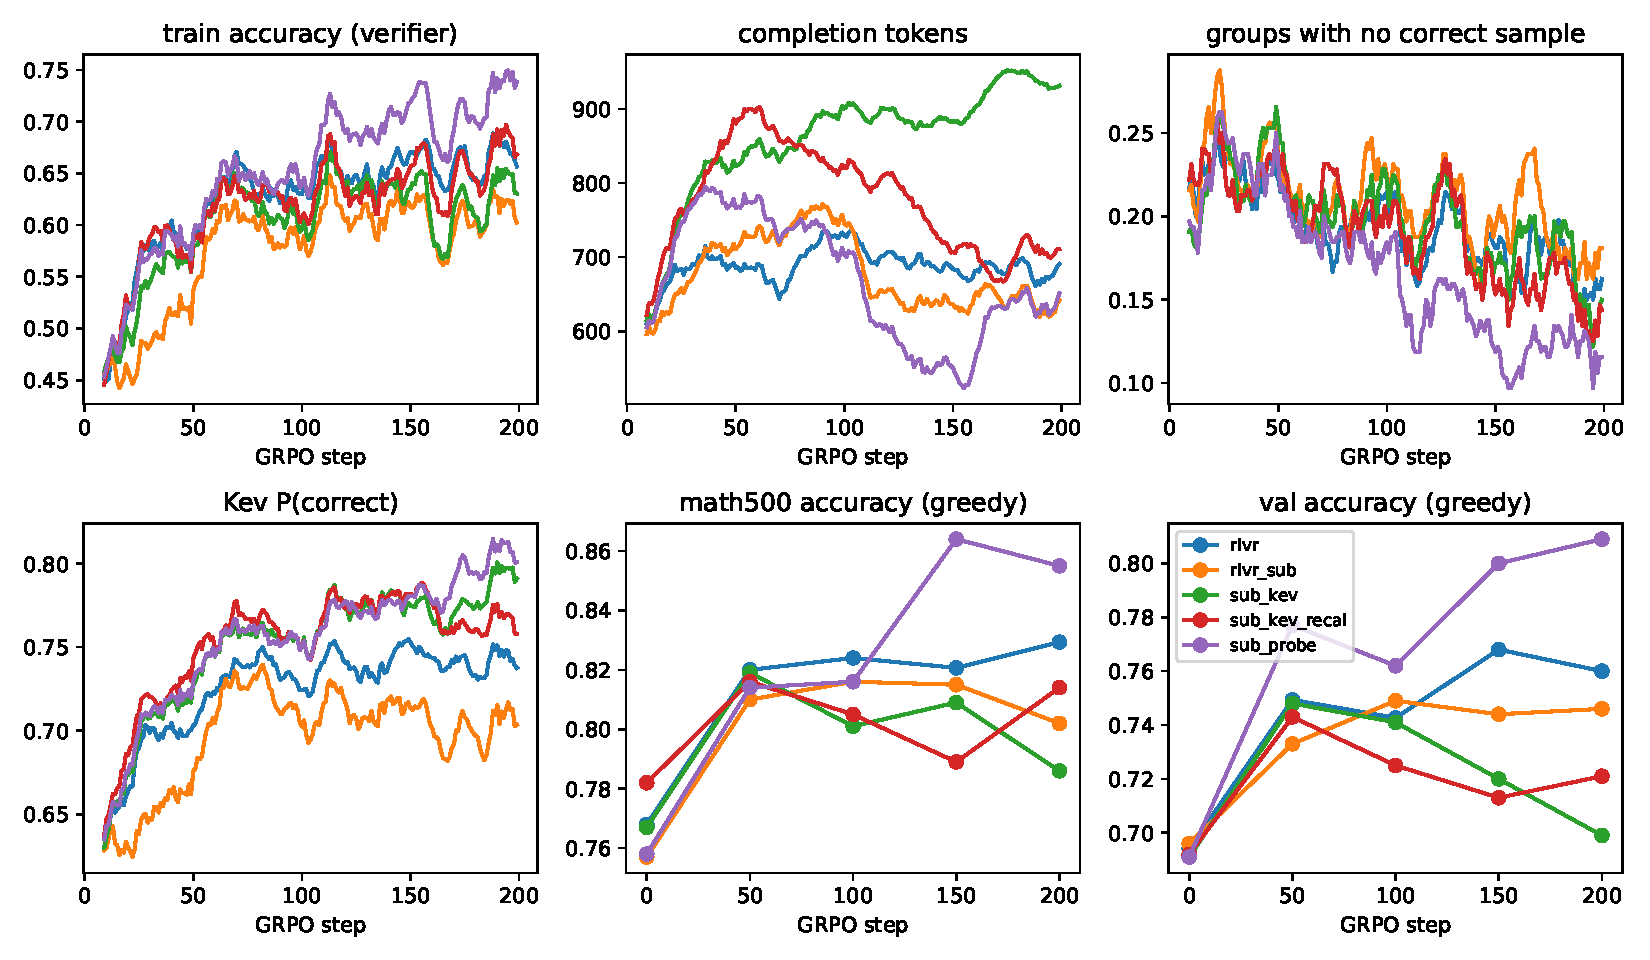
\includegraphics[width=\linewidth]{../../experiments/part3b_labels/results/training_curves.pdf}
\caption{Training curves (seed mean): verifier accuracy of all training completions (labelled or not), completion
tokens, share of groups with no correct completion and \kev{}'s $\pc$ on the training completions (10-step moving
averages), and greedy accuracy on MATH-500 and the validation set every 50 steps.}
\label{fig:sub-curves}
\end{figure}

\paragraph{Evaluation noise.} Across the \NUM{szruns_math500} runs in this comparison, the base model's MATH-500
accuracy at step 0 ranges from \NUM{szmin_math500}\% to \NUM{szmax_math500}\%, and a run's accuracy changes by
\NUM{lecabs_math500} points on average between its evaluations at steps 150 and 200. The final weights of each run are
evaluated twice on MATH-500, both times greedily: at step 200 with the periodic evaluations, and in the final
evaluation. The two results differ by \NUM{rptabs_math500} points on average and by up to \NUM{rptmax_math500}
(\NUM{rptruns_math500} runs).

\subsection{Does the judge pay for repetition?}\label{sec:res-repeat}

After the GRPO runs we tested whether \kev{} pays for what the policies of \texttt{sub\_kev} and
\texttt{sub\_kev\_recal} write after their first answer, with the probe of Part II (\file{dcjev/llm/repeat_probe.py};
Table~\ref{tab:repeat-probe}). \texttt{sub\_kev}'s policy restates its conclusion again and again;
\texttt{sub\_kev\_recal}'s solves the problem again in nearly the same words, like Part II's policies with \kev{} in
the reward. We cut the final MATH-500 solutions of seed 1 that repeat lines after their first answer, as if the policy
had stopped there. Solutions that repeat before their first answer, or whose first answer differs from their last,
were left out (\NUM{rpskip_subkev} and \NUM{rpskip_subrecal}). No edit changes the answer the verifier reads.

The part after the first answer raises the released \kev{}'s $\pc$, \texttt{sub\_kev}'s fill-in reward, by
\NUM{rpkevc_cutsubkev_1} \ci{\NUM{rpkevclo_cutsubkev_1}}{\NUM{rpkevchi_cutsubkev_1}} on right answers and by
\NUM{rpkevc_cutsubkev_0} \ci{\NUM{rpkevclo_cutsubkev_0}}{\NUM{rpkevchi_cutsubkev_0}} on wrong ones. On
\texttt{sub\_kev\_recal}'s solutions it raises it by \NUM{rpkevc_cutsubrecal_1}
\ci{\NUM{rpkevclo_cutsubrecal_1}}{\NUM{rpkevchi_cutsubrecal_1}} and \NUM{rpkevc_cutsubrecal_0}
\ci{\NUM{rpkevclo_cutsubrecal_0}}{\NUM{rpkevchi_cutsubrecal_0}}, for \NUM{rpkevcup_cutsubrecal_0} of the wrong ones.
Repetition as such is worth little: written into the base policy's solutions, it raises \kev{}'s $\pc$ by
\NUM{rpkevc_end3_1} on right answers and changes it by \NUM{rpkevc_end3_0} on wrong ones. So on the unlabelled
completions the fill-in reward paid for what these policies learned to write after their first answer, most of all on
wrong answers, to which the verifier would have given nothing. The probe scores with the released head. The head of
\texttt{sub\_kev\_recal} was refitted during training, and its own preference at the end of the run is not measured
here. The AR judge, which no condition used, rates \texttt{sub\_kev\_recal}'s solutions higher with the part after the
first answer (\NUM{rparc_cutsubrecal_1} on right answers) but \texttt{sub\_kev}'s endless restatements lower
(\NUM{rparc_cutsubkev_1} on right answers, \NUM{rparc_cutsubkev_0} on wrong ones).

\begin{table}[t]
\centering\small
\begin{tabular}{@{}lccccccc@{}}
\toprule
 & solutions & \multicolumn{2}{c}{\kev{} $\pc$} & \multicolumn{2}{c}{\kev{} $\pg$} & \multicolumn{2}{c}{AR $P_{\mathrm{a}}$} \\ \cmidrule(lr){3-4}\cmidrule(lr){5-6}\cmidrule(l){7-8}
 & right / wrong & right & wrong & right & wrong & right & wrong \\ \midrule
\multicolumn{8}{@{}l}{\emph{base policy's solutions, repetition added}} \\
\quad last two paragraphs twice more & 2436 / 1537 & $+$0.012 & $-$0.002 & $+$0.007 & $-$0.006 & $+$0.037 & $+$0.012 \\
\quad written twice & 2436 / 1564 & $+$0.012 & $-$0.003 & $+$0.006 & $-$0.004 & $+$0.029 & $+$0.007 \\
\multicolumn{8}{@{}l}{\emph{repeating final solutions of GRPO runs, as written against cut after the first answer}} \\
\quad \texttt{sub\_kev}, seed 1 & 351 / 66 & $+$0.031 & $+$0.049 & $+$0.016 & $+$0.031 & $-$0.018 & $-$0.074 \\
\quad \texttt{sub\_kev\_recal}, seed 1 & 318 / 81 & $+$0.059 & $+$0.110 & $+$0.030 & $+$0.095 & $+$0.034 & $+$0.034 \\
\bottomrule
\end{tabular}

\caption{What repetition is worth to the judges (the probe of Part II): P(with the repetition) minus P(without), on the
solutions the verifier accepts (right) and rejects (wrong), with the number of each. Top: the base policy's solutions
of Part II's judge study, with repetition added. Bottom: the final MATH-500 solutions of seed 1 that repeat lines, as
written against cut after their first answer. The released \kev{}'s $\pc$ and $\pg$ and the AR judge's
$P_{\mathrm{a}}$; intervals in the text resample problems.}
\label{tab:repeat-probe}
\end{table}
